\section{The Salience-biased Affinity Propagation (SAP) Summarizer}
\label{sec:sap}

We now present our first streaming summarization model, the salience-biased
affinity propagation (SAP) summarizer. The SAP summarizer predicts sentence
salience with respect to a query $\query$, and integrates these predictions
into a clustering based multi-document summarization system. We demonstrate
that combining salience with clustering produces more relevant summaries
compared to baselines using clustering or salience alone.  Our experiments
suggest that this is because our system is better able to adapt to dynamic
changes in input volume that adversely affect methods that use redundancy as a
proxy for salience. 

In addition to the tight integration between clustering and salience
prediction, our approach also exploits knowledge about the event to determine
salience. Thus, salience represents both how typical a sentence is of the event
category (e.g., industrial accident, hurricane, riot) and whether it specifies
information about this particular event.  Our feature representation includes a
set of language models, one for each event category, to measure the typicality
of the sentence with regard to the current event, the physical distance of
mentioned locations from the center of the event, and the change in word
frequencies over the time of the event.  While we evaluate these features in
the domain of disasters, this approach is applicable to any streaming
summarization task.

We evaluate the SAP summarizer with two main experiments. First, we present the
results of our model in the TREC 2014 Temporal Summarization shared-task
\citep{aslam2014}, where the SAP summarizer achieved top performance on the
main evaluation metric ($\harm$), and was also shown to have higher precision
relative to other participant systems.  Second, we perform our own independent
evaluation, and show our approach achieves a statistically significant
improvement in \rouge~scores compared to multiple baselines in addition to the
expected gain and comprehensiveness metrics.  We also perform a feature
ablation experiment to see which features are most important in our salience
estimation component.

\subsection{Summarization Model}
\label{sec:methods}

\begin{algorithm}[t]
    \KwIn{
        query string $\query$, 
        query category $\category$, 
        stream $\sentstream$, 
        period of interest $(\poestart, \poestop)$}
    \KwOut{update summary $\updateSummary$~\\~\\}
    
    \tcc{Initialize empty update summary and system start time.}
    $\updateSummary \gets \left[ \right]$ \label{alg:initstart}\\
    $t \gets 1$\\
    $\systs_0 \gets \poestart$ \\
    $\systs_1 \gets \poestop + \dhour$ \label{alg:initstop} \\
\While{$\systs_t < \poestop$}{

    \fcolorbox{red}{red!20!}{\begin{minipage}{0.9\textwidth}
    \tcc{Predict salience (\autoref{sec:salpred})}\end{minipage}}\\
    $\spredsals_t \gets \left[ \right]$  \label{alg:salstart}\\
    \For{$\ssent_i \in \sentstream_{\systs_{t-1}:\systs_t}$}{
   $\spredsals_t \gets \spredsals \oplus \left[\salmodf{\featf{\ssent_i,\query, \category}}\right]$ \label{alg:salstop}\\
    }
    \fcolorbox{green}{green!20!}{\begin{minipage}{0.9\textwidth}
\tcc{Select exemplars with SAP clustering (\autoref{sec:exsel})}\end{minipage}}\\

   $\Exemplars_t \gets \operatorname{APCluster}(\sentstream_{\systs_{t-1}:\systs_t}, \spredsals_t)$ \label{alg:clust} \\ 
    \fcolorbox{blue}{blue!20!}{\begin{minipage}{0.9\textwidth}
\tcc{Select next updates (\autoref{sec:upsel})}\end{minipage}}\\
    $\updateSummary_t \gets \operatorname{FilterRedundant}(\Exemplars_t, \updateSummary)$   \label{alg:filter} \\
    \For{$\supdate \in \updateSummary_t$}{
     $\updateSummary \gets \updateSummary \oplus \left[\left(\supdate,\systs_t\right)\right]$ \label{alg:add} \\
    }
$\systs_{t+1} \gets \systs_t + \dhour$\\
$t \gets t + 1$
}
\caption{Salience-biased Affinity Propagation (SAP) Summarizer}
\label{alg:clustsum}
\end{algorithm}


The summarizer takes as input the query string $\query$ and category
$\category$, as well as the period of interest, ($\poestart, \poestop$), i.e.,
the time period of the stream on which to run the summarizer. The summarizer
works by incrementing the system time in hourly batches, processing the newly
observed sentences, and selecting some of them to be updates, which are then
added to the update summary. When the system time exceeds $\poestop$, the
summarizer terminates, returning the completed update summary.

Pseudo-code for the SAP summarizer is shown in \autoref{alg:clustsum}.  The
algorithm starts with an empty update summary $\updateSummary$ and initial
system time $\systs_1 = \poestart + \dhour$ (\hyperref[alg:clustsum]{Alg.
\ref{alg:clustsum} lines \ref{alg:initstart}--\ref{alg:initstop}}).  System
time is incremented in hourly intervals, i.e. $\systs_{t} - \systs_\tmo =
\dhour$.  At each time $\systs_t$, we process the sentences that entered the
stream in the last hour, $\sentstream_{\systs_\tmo:\systs_t}$, by performing
the following actions:
\begin{enumerate}
    \item predict the salience $\spredsal_i$ of sentences $\ssent_i \in
\sentstream_{\systs_\tmo:\systs_t}$
(\hyperref[alg:clustsum]{Alg. \ref{alg:clustsum} lines
\ref{alg:salstart}--\ref{alg:salstop}}, \autoref{sec:salpred}),
    \item select a set of exemplar sentences $\Exemplars_t \subset
\sentstream_{\systs_\tmo:\systs_t}$ by combining
affinity propagation clustering with salience predictions
(\hyperref[alg:clustsum]{Alg. \ref{alg:clustsum} line \ref{alg:clust}},
\autoref{sec:exsel}),
    \item add the most novel and salient exemplars,
$\updateSummary_{\systs_t}$, to the update summary $\updateSummary$
(\hyperref[alg:clustsum]{Alg. \ref{alg:clustsum} lines
\ref{alg:filter}--\ref{alg:add}}, \autoref{sec:upsel}).
\end{enumerate}
Once the system time $\systs_t$ exceeds the period of interest (i.e., $\systs_t
> \poestop$), the summarizer returns collected set of updates $\updateSummary$
as the summary of the event.

%\subsection{\colorbox{red!20!}{Salience Estimation}}
\subsection{{Salience Estimation}}
\label{sec:salpred}

\subsubsection{Model}

Given a sentence $\ssent \in \sentstream_{\systs_\tmo:\systs_t}$ from the
current hourly batch, the salience estimation model determines how important or
relevant it's content is with respect to the query. Since we do not have manual
assessments of query-sentence salience for the overwhelming majority of the
sentences in the KBA Stream Corpus, we rely on an automatic measure for
determining the salience targets we wish to predict.

Let $\snuggets$ be a timestamped collection of reference nuggets for query
$\query$. We define the salience of a sentence $\ssent$ with respect to
$\query$ to be the degree to which it reflects an event's reference nuggets,
which we define as its maximum nugget similarity,
\begin{align}
\salop{\ssent, \query} = \max_{\ntuple{i} \in \snuggets} 
\simop{\ssent, \snugget_i}. \label{eq:salience}
\end{align}

We implement the similarity function using the cosine-similarity of
latent-space vectors associated with $\ssent$ and $\snugget_j$ using weighted
matrix factorization (WMF) \citep{srebro2003,guo2012}. Given a term-sentence
matrix $\tsmat \in \reals^{\sdimw \times \sdims}$ where $\tsmat_{i,j}$ is the
TF-IDF weight of term $i$ in sentence $j$, WMF finds a low-rank approximation
$\wproj^\T\sproj \approx \tsmat$ where $\wproj \in \reals^{\sdiml \times
\sdimw}$ and $\sproj \in \reals^{\sdiml \times \sdims}$ are projection matrices
into the latent term and document  spaces respectively.  The projection
matrices are found by minimizing the weighted reconstruction error of $\tsmat$
under a least squares objective, i.e.,
\[
    \obj{\wproj,\sproj} = 
      \sum_{i=1}^\sdimw \sum_{j=1}^\sdims
        \wmat_{i,j} \left( 
          \tsmat_{i,j} - \left(\wproj^\T\sproj\right)_{i,j}
        \right)^2 + \textrm{reg.}
\] 
Following \cite{guo2012}, we set the weight $\wmat_{i,j}$ to 
\[ 
    \wmat_{i,j} = \begin{cases} 
        0.01 & \textrm{if $\tsmat_{i,j} = 0$,}\\
        1 & \textrm{otherwise}
   \end{cases}
\] 
which focuses the reconstruction on non-zero entries in $\tsmat$. The intuition
here is that $\tsmat$ is sparse so error in modeling the 0 entries, which we
care least about, will dominate the loss. By down-weighting those entries, the
projection matrices must better represent how terms are positively associated
to the documents they occur in.\footnote{WMF is similar to latent semantic
analysis (LSA) \citep{dumais1988} which uses a truncated singular-value
decomposition to obtain term and sentence projections but does not reweight
non-zero entries.  Interestingly, WMF is also similar to the global vector
(GloVe) embedding method \citep{pennington2014glove} which minimizes a weighted
least squares objective of a term-by-term log cooccurrence matrix.} Let
$\latf{\ssent},\latf{\snugget} \in \reals^\sdimw$ be projections into TF-IDF
weighted bag-of-words space of $\ssent$ and $\snugget$ respectively. The
similarity of $\ssent$ and $\snugget$ then is defined as, 
\begin{align}
\simop{\ssent,\snugget} =
\cossim{\wproj \cdot \latf{\ssent}, \wproj \cdot \latf{\snugget}}. 
\label{eq:semsim} 
\end{align}

Since the summarizer will not have knowledge of the reference summary
$\snuggets$ at test time, we must estimate \autoref{eq:salience} without it.
To that end, we fit a regression model $\salmodf{\cdot}$ to estimate the
salience of a sentence with respect to the query, i.e., 
\begin{align}
\salop{\ssent, \query} \approx \salmodf{\featf{\ssent,\query,\category}}
\label{eq:approxsal} 
\end{align} 
using features, $\featf{\ssent,\query,\category}$, of the sentence, query, and
query category.

We opt to use a Gaussian process (GP) regression model \citep{rasmussen2005}
with a radial basis function (RBF) kernel for the salience prediction task.
Our features fall naturally into five groups (which we describe below) and we
use a separate RBF kernel for each, using the sum of each feature group RBF
kernel as the final input to the GP model.

Given our feature representation of the input sentences, we need only target
salience values for model learning. For each query event in our training data,
we sample a set of sentences and  each sentence's salience is computed
according to \autoref{eq:salience}. This results in a training set of sentences
with their feature representations and target salience values, to which we fit
the salience estimator.

\subsubsection{Features} \label{sec:features}

We want our model to be predictive of sentence salience across different event
instances so we avoid event-specific lexical features.  Instead, we extract
features such as language model scores, geographic relevance, and temporal
relevance from each sentence; these features in our initial model development
were consistently helpful across specific event instances and categories.

\textbf{Basic Features} We employ several basic features that have been used
previously in supervised models to rank sentence salience
\citep{kupiec1995trainable,conroy2001}.  These include sentence length, the
number of capitalized words normalized by sentence length, document position,
and number of named entities.  The data stream comprises text extracted from
raw html documents; these features help to down-weight sentences that are not
content (e.g. web page titles, links to other content) or more heavily weight
important sentences (e.g., that appear in prominent positions such as paragraph
initial or article initial).

\textbf{Query Features} Query features measure the relationship between the
sentence and the event query and category.  These include the number of query
words present in the sentence in addition to the number of event category
synonyms, hypernyms, and hyponyms using WordNet \citep{miller1995wordnet}.  For
example, for event category \emph{earthquake},  we match sentence terms
``quake'', ``temblor'', ``seism'', and ``aftershock''.

\textbf{Language Model Features}\label{subsubsec:lm} Language models allow us
to measure the likelihood of producing a sentence from a particular source.  We
consider two different language models to obtain features.  The first model is
estimated from a corpus of generic news articles (we used the 1995-2010
Associated Press section of the Gigaword corpus \citep{graff2003english}).
This model is intended to assess the general writing quality (grammaticality,
word usage) of an input sentence and helps our model to select sentences
written in the newswire style.  

The second model is estimated from text specific to our event categories.  For
each event category we create a corpus of related documents using pages and
subcategories listed under a related Wikipedia category. For example, the
language model for event category \textit{earthquake} is estimated from
Wikipedia pages under \emph{Category:Earthquakes}.  \autoref{tab:queries} lists
the event categories for each of the events in our dataset. These models are
intended to detect sentences similar to those appearing in summaries of other
events in the same category (e.g., most earthquake summaries are likely to
include higher probability for ngrams including the token `magnitude').  While
we focus our system on the language of news and disaster, we emphasize that the
use of language modeling can be an effective feature for multi-document
summarization for other domains that have related text corpora.

We use the SRILM toolkit \citep{stolcke2002srilm} to implement a 5-gram
Kneser-Ney model for both the background language model and the event category
specific language models. For each sentence we use the average token log
probability under each model as a feature.

\textbf{Geographic Relevance Features} The events in our corpus are all
phenomena that affect some part of the world.  Where possible, we would like to
capture a sentence's proximity to the event, i.e. when a sentence references a
location, it should be close to the geographic area of the event.

There are two particular challenges to using geographic features in our present
setting. First, we do not know where the event is, and second, most sentences
do not contain references to a location. We address the first issue by
extracting all locations (using contiguous token spans tagged with a location
tag under a named-entity tagger) from documents relevant to the event at the
current hour (i.e. $\sdoc_i \in \docstream_{\systs_\tmo:\systs_t}$) and looking
up their latitude and longitude using a publicly available geo-location
service.  Since the documents are at least somewhat relevant to the event, we
assume in aggregate the locations should give us a rough area of interest.  The
locations are clustered and we treat the resulting cluster centers as the event
locations for the current time.\footnote{The great-circle distance
(\url{https://en.wikipedia.org/wiki/Great-circle_distance}), which is the
shortest arc between two points projected onto the surface of a sphere, is used
as the distance metric for clustering. Clustering is done with affinity
propagation clustering.}

The second issue arises from the fact that the majority of sentences in our
data do not contain explicit references to locations.  Our intuition is that
geographic relevance is important in the disaster domain, and we would like to
take advantage of the sentences that do have location information present. To
make up for this imbalance, we instead compute an overall location for the
document and derive geographic features based on the document's proximity to
the event in question. These features are assigned to all sentences in the
document.

Our method of computing document-level geographic relevance features is as
follows. Using the locations in each document, we compute the median distance
to the nearest event location. Because document position is a good indicator of
importance we also compute the distance of the first mentioned location to the
nearest event location. All sentences in the document take as features these
two distance calculations. Because some events can move, we also compute these
distances to event locations from the previous hour.

\textbf{Temporal Relevance Features} As we track events over time, it is likely
that the coverage of the event may die down, only to spike back up when there
is a breaking development.  Identifying terms that are ``bursty,'' i.e.
suddenly peaking in usage, can help to locate novel sentences that are part of
the most recent reportage and have yet to fall into the background.

We compute the IDF\textsubscript{$t$} for each hour sub-sequence,
$\sentstream_{\systs_\tmo:\systs_t}$. For each sentence $\ssent \in
\sentstream_{\systs_\tmo:\systs_t}$, the average TF-IDF\textsubscript{$t$} is
taken as a feature. Additionally, we use the difference between average
TF-IDF\textsubscript{$t$} and average TF-IDF\textsubscript{$t-i$}  for $i \in
\{1, \ldots, 24\}$ to measure how the TF-IDF scores for the sentence have
changed over the last 24 hours, i.e. we keep the sentence term frequencies
fixed and compute the difference in IDF. Large changes in IDF value indicate
the sentence contains bursty terms.  We also use the time (in hours) since the
event started as a feature.

%\subsection{\colorbox{green!20!}{Affinity Propagation Clustering}}
\subsection{{Affinity Propagation Clustering}}
\label{sec:exsel}

Once we have predicted the salience for a batch of sentences, we must now
select a set of update candidates, i.e. sentences that are both salient and
representative of the current batch. To accomplish this, we combine the output
of our salience prediction model with the affinity propagation clustering
algorithm \citep{frey2007}.

Affinity propagation (AP)  identifies a subset of data points as exemplars and
forms clusters by assigning the remaining points to one of the exemplars.  Let
\[
    \cin = \left\{\ssent_1,\ldots,\ssent_\cinsize \right\}
\]
be a set of $\cinsize$ data points to be clustered and let 
\[
    \exemplars = \left[\exemplar_1,\ldots,\exemplar_\cinsize \right]
\]
be a vector of corresponding exemplar assignments, i.e.  $\exemplar_i \in
\{1,\ldots,\cinsize\}$ and $\exemplar_i = k$ means that $\ssent_k$ is the
exemplar for $\ssent_i$.

AP attempts to maximize the constrained net similarity objective,
\[ \obj{\exemplars} = e^{\Big(
    \sum_{i=1}^\cinsize \csim\left(\ssent_i,\ssent_{\exemplar_i}\right) 
    + \sum_{k=1}^\cinsize \log \apcons_k(\exemplars) 
\Big)}
\]
where $\csim\left(\ssent_i, \ssent_{\exemplar_i}\right) \in \reals$ measures
the affinity of $\ssent_i$ for its exemplar $\ssent_{\exemplar_i}$ and 
\[
    \apcons_k(\exemplars) = \begin{cases} 
    0 & \textrm{$\exemplar_k \ne k$ but $\exists i: \exemplar_i = k$ } \\ 
    1 & \textrm{otherwise}      \end{cases}
\] 
expresses the constraint that if $\ssent_k$ is some point's exemplar, it must
be its own exemplar, i.e. all clusters must have one exemplar. The affinities
can be interpreted as a log-probabilities of the exemplar-assignments, i.e.
$p(\exemplars) = \frac{\obj{\exemplars}}{ \sum_{\boldsymbol{\exemplars^\prime }
} \obj{\boldsymbol{\exemplars^\prime }} }.$ \cite{frey2007} show the net
similarity objective can be viewed as a factor graph and an optimal
configuration can be found using max-product message passing.  For the affinity
function $\csim$, we use
\[ 
    \csim\left(\ssent_i, \ssent_{\exemplar_i}\right) = \begin{cases}
        \salmodf{\featf{\strmSent_i,\query,\category}} & 
            \textrm{if $i = \exemplar_i$ }\\
         \simop{\ssent_i,\ssent_{\exemplar_i}} & \textrm{otherwise}
\end{cases}
\]
where $\salmodf{\featf{\ssent_i,\query,\category}}$ is the salience estimate of
sentence $\ssent_i$ (\autoref{eq:approxsal}) and $\simop{\ssent_i,
\ssent_{\exemplar_i}}$ is the WMF-based similarity method
(\autoref{eq:semsim}).

AP has several useful properties relevant to our stream summarization task.
Chiefly, the number of clusters $k$ is not a model hyper-parameter. Given that
our task requires clustering many batches of data with potentially large
variations in the volume of data per batch, searching for an optimal $k$ would
be computationally prohibitive. With AP, $k$ is determined by the
self-affinity, $\csim(\ssent_i,\ssent_i)$, of the data,  with lower overall
values of $\csim(\ssent_i,\ssent_i)$ yielding a smaller number of clusters.
When the volume of input is high but the salience predictions are low, the
self-affinity term will guide AP toward a solution with fewer clusters;
\textit{vice-versa} when input is very salient on average but the volume of
input is low. The adaptive nature of our model differentiates our method from
most other update summarization systems.

In the summarization pipeline, given a batch of sentences
$\sentstream_{\systs_\tmo:\systs_t}$ and their salience estimates
$\spredsals_t$, we run the AP clustering algorithm and obtain the set of
exemplars $\Exemplars_t = \apop(\sentstream_{\systs_\tmo:\systs_t},
\spredsals_t)$. The exemplars $\Exemplars_t$ are then passed to a redundancy
filtering stage which we describe next.

%\subsection{\colorbox{blue!20!}{Redundancy Filtering and Update Selection}}
\subsection{{Redundancy Filtering and Update Selection}}
\label{sec:upsel}

The exemplar sentences from the exemplar selection stage are the most salient
and representative of the input for the current hour. However, we need to
reconcile these sentences with updates from the previous hours to ensure that
the most salient and least redundant  updates are selected. To ensure that only
the most salient updates are selected we apply a minimum salience threshold;
after exemplar sentences have been identified, any exemplars whose salience is
less than $\sapsalth$ are removed from consideration. 

Next, to prevent adding updates that are redundant with previous output
updates, we filter out exemplars that are too similar to previous updates.  The
exemplars are examined sequentially in order of decreasing salience and  a
similarity threshold is applied, where the exemplar is ignored if its maximum
semantic similarity to any previous updates in the summary is greater than
$\sapsimth$.  Exemplars that pass these thresholds (indicated as
$\updateSummary_t$ in \hyperref[alg:clustsum]{Alg. \ref{alg:clustsum} line
\ref{alg:filter}}) are selected as updates and added to the summary.

\subsection{TREC 2014 Experiments and Results}

\begin{table}[t]
\centering
\begin{tabular}{cccccc}
\toprule
TeamID & RunID &$n\mathbb{E}[\gain](\updateSummary)$ & $\comp(\updateSummary)$ & $\comp_L(\updateSummary)$ & $\mathcal{H}_L(\updateSummary)$ \\
\midrule
\textbf{cunlp} & \textbf{2APSal} & 0.0631 & 0.3220 & 1.2068 & \textbf{0.1162} \\
BJUT & Q1 & \textbf{0.0657} & 0.4088 & 1.1491 & 0.1110\\
BJUT & Q2 & 0.0632 & 0.3979 & 1.1669 & 0.1091\\
BJUT & Q0 & 0.0632 & 0.3979 & 1.1669 & 0.1091\\
uogTr & uogTr2A & 0.0467 & 0.4453 & 1.2322 & 0.0986\\
uogTr & uogTr4AC & 0.0347 & 0.4539 & 1.2751 & 0.0793\\
uogTr & uogTr4ARas & 0.0387 & 0.3691 & 1.2328 & 0.0772\\
IRIT & KW30H5NW3600 & 0.0383 & 0.3521 & 1.2221 & 0.0723\\
IRIT & KW30H5NW300 & 0.0378 & 0.3538 & 1.2208 & 0.0714\\
uogTr & uogTr4A & 0.0281 & \textbf{0.4733} & 1.2522 & 0.0677\\
\midrule
\multicolumn{2}{c}{\textit{average}} & 0.0327 & 0.3615 & 1.2943 & 0.0620\\
\midrule
IRIT & KW80H5NW3600 & 0.0289 & 0.3764 & 1.2191 & 0.0604\\
IRIT & KW30H10NW300 & 0.0298 & 0.3780 & 1.2617 & 0.0602\\
\textbf{cunlp} & \textbf{1APSalRed} & 0.0325 & 0.3058 & 1.1507 & 0.0602\\
IRIT & KW80H5NW300 & 0.0285 & 0.3806 & 1.2164 & 0.0596\\
ICTNET & run3 & 0.0531 & 0.1081 & 0.7004 & 0.0530\\
BUPT\_PRIS & Cluster4 & 0.0155 & 0.2692 & 1.9140 & 0.0508\\
IRIT & KW80H10NW300 & 0.0225 & 0.4012 & 1.2621 & 0.0503\\
BUPT\_PRIS & Cluster3 & 0.0115 & 0.3380 & 1.9165 & 0.0407\\
\textbf{cunlp} & \textbf{3AP} & 0.0174 & 0.4265 & 1.3689 & 0.0403\\
ICTNET & run2 & 0.0418 & 0.0934 & 0.6266 & 0.0311\\
BUPT\_PRIS & Cluster2 & 0.0059 & 0.3728 & 1.9170 & 0.0222\\
ICTNET & run4 & 0.0079 & 0.4070 & 1.2364 & 0.0178\\
ICTNET & run1 & 0.0070 & 0.4090 & 1.2314 & 0.0160\\
BUPT\_PRIS & Cluster1 & 0.0033 & 0.4369 & \textbf{1.9175} & 0.0127\\
\bottomrule
\end{tabular}
\caption{Official TREC 2014 Temporal Summarization shared-task results using
manual update/nugget matches.}
\label{tab:trec2014}
\end{table}


We submitted three different model variations to the 2014 TREC Temporal
Summarization shared-task \citep{aslam2015}. The models were submitted under
the Team ID \textit{cunlp} and given the following Run IDs:
\begin{enumerate}
\item 1APSalRed --- the SAP summarizer where salience predictions are penalized
by similarity to prior updates. Let $\spredsal_k =
\salmodf{\featf{\supdate_k,\query,\category}}$ for each update in
$\updateSummary$. The salience estimate for a new sentence $\ssent_i$ is
$\salmodf{\featf{\ssent_i,\query,\category}} - \sum_{\utuple{k} \in
\updateSummary} \spredsal_k \cdot \simop{\ssent_i,\supdate_k}$. 
\item 2APSal --- the SAP summarizer.
\item 3AP --- the summarizer with no salience estimation, all non-singleton
 exemplars are passed on to the redundancy filter and update selection
stage.
\end{enumerate}

We use the 10 TREC 2013 events to train/tune our submitted models.  Three of
the events were selected at random as a development set. All system salience
and similarity threshold parameters are tuned on the development set to
maximize \rouge-2 F1 scores with respect to the reference summaries
$\snuggets$.  We fit separate salience models using 1,000 sentences randomly
sampled from each of the seven remaining TREC 2013 query events using its
associated document stream.  When predicting the salience for a new sentence at
test time, we use the average prediction of all seven models. 


Participant systems were run on 15 query events and associated document streams
curated for the evaluation.  Updates from the participant systems were pooled
and manually matched to reference nuggets by NIST assessors. These matches were
used to compute the  shared-task evaluation metrics (\autoref{sec:methods}):
normalized expected gain, $\nEG(\updateSummary)$, comprehensiveness
$\comp(\updateSummary)$, latency-penalized comprehensiveness
$\comp_\latency(\updateSummary)$, and the overall track evaluation measure, the
harmonic mean $\harm_\latency(\updateSummary)$ of the latency-penalized
$\nEG(\updateSummary)$ and $\comp(\updateSummary)$ variants.

\begin{figure*}
\begin{tabular}{|l m{15cm}|}
\multicolumn{2}{c}{\textbf{Hurricane Sandy}}\\
\hline
\hline
\small
\tabitem & The forecast map shows Sandy reaching eastern Cuba by early Thursday 
  before heading to the Bahamas.\\
\small
\tabitem & Jamaica's government issued a hurricane warning on Tuesday morning and 
    announced schools would be closed on Wednesday.\\
\small
\tabitem  & \small Dangerous flash floods and mudslides set off by Sandy were a threat for the
   island of roughly 2.7 million inhabitants, Jamaica's meteorological service
   said.\\
\small
\tabitem  & \small A few reliable forecast models bring Sandy close enough to the coast to 
produce heavy rains, strong winds and beach erosion.\\
\small
\tabitem  & \small Max winds are 65 mph with strengthening to a hurricane expected in the next
 12 to 18 hours.\\
\small
\tabitem & \small The two international airports, as well as schools and businesses, 
         will remain closed today until the hurricane warning, which is now in
         effect for the island, is lifted. \\
\hline
%%at 11 a.m., sandy was in the caribbean about 65 miles south of kingston , jamaica , moving north at 13 mph with sustained winds of 80 mph.
%%"""""""we heard on the radio that the hurricane was coming this way,"""""""" he said in the poor kingston community of standpipe, situated next to one of the debris-clogged gullies that crisscross the capital."""""""
\end{tabular}

~\\
~\\
\begin{tabular}{|l m{15cm}|}
\multicolumn{2}{c}{\textbf{2012 Pakistan Garment Factory Fires}}\\
\hline
\hline
%\small
%\tabitem &\small  Medical officials said that some had died of suffocation while others
%         were burnt alive as the fire took hold. \\
\small
\tabitem & \small The fire broke out when people in the building were trying to start 
         their generator after the electricity went out. \\
\small
\tabitem & \small Pakistani television showed pictures of what appeared to be a 
         three-story building with flames leaping from the top-floor windows 
         and smoke billowing into the night sky. \\
\small
\tabitem & \small The people went to the back side of the building but there was no 
         access, so we had to made forceful entries and rescue the people, 
         said Numan Noor, a firefighter on the scene. \\
\small
\tabitem & \small ``We have recovered 63 bodies, including three found when we reached 
         the basement of the building,'' Karachi fire chief Ehtesham Salim told
         AFP on Wednesday. \\
\small
\tabitem & \small Salim added that the blaze was Karachi’s ``biggest fire in terms of 
         deaths in decades.'' \\
\small
\tabitem & \small The garment trade as a whole is vital to Pakistan’s shaky economy. \\
\hline
\end{tabular}

~\\
~\\
\begin{tabular}{|l m{15cm}|}
\multicolumn{2}{c}{\textbf{2012 Romanian Protests}}\\
\hline
\hline
\small
\tabitem & \small Clashes between riot police and demonstrators have also erupted in 
         the Romanian capital Bucharest for a third day in a row. \\
\small
\tabitem & \small BOC urged Romanians to understand that tough austerity measures are 
         needed to avoid a default. \\
\small
\tabitem & \small More than 1,000 protesters rallied in Bucharest's main university 
         square, blocking traffic. \\
\small
\tabitem & \small Bucharest : a Romanian medical official says 59 people suffered 
         injuries as days of protests against the government and austerity 
         measures turned violent. \\
\small
\tabitem & \small Most Romanians agree that only fundamental reform can save the 
         country's ailing and corrupt system. \\
\small
\tabitem & \small Many Romanians feared this would only increase corruption and create 
        a further divide between the classes, leading to a two-tier system in
        which only the wealthy would be able to afford care. \\
\hline
\end{tabular}

\caption{\textsc{SAP} summary excerpts.}
\label{fig:sapsummaries}
\end{figure*}


To give a qualitative flavor of our produced summaries, we show excerpts of two
summaries produced by the 2APSal, i.e. SAP, model, in
\autoref{fig:sapsummaries}.  Results from the official TREC 2014 Temporal
Summarization shared-task are shown in \autoref{tab:trec2014}. We see that our
2APSal model had the highest overall $\harm_\latency(\updateSummary)$. It was
also one of the most precise models along with BJUT runs Q1, Q2, and Q0. The
2APSal and the BJUT runs return far fewer updates on average while still
managing to include updates that matched to nuggets. The 2APSal run returned
381.4 updates per query on average while the overall track average was 8,528.55
updates per query on average. 

When we look at 3AP, which had no salience component, it had higher recall
(i.e. comprehensiveness) than 2APSal but was much less precise, returning 5,967
updates on average. This suggests that the salience estimation was important
for guiding the summarizer. 

The performance of 1APSalRed was between 3AP and 2APSal. The redundancy penalty
meant that the average self-similarities were flatter than those of 2APSal
yielding more diverse updates, which were not as likely to be matched to
ground-truth nuggets, and therefore hurting the expected gain metrics.

All three of our proposed models had a latency-penalized comprehensiveness,
$\comp_\latency(\updateSummary)$, above one ($1.1507 - 1.3689$). Values above
one indicate the average update that matched a nugget was selected before that
information made it into Wikipedia (and confusingly getting a latency reward
for early returns). In this case our proposed model was finding nugget
information around three to five hours ahead of its publication in Wikipedia.  

\subsection{Automatic Experiments}

Independent of the official TREC shared-task evaluation we also perform our own
experiments using automatically computed metrics.  In particular, we compute
\rouge~with respect to the reference summaries $\snuggets$, and expected gain
and comprehensiveness computed using automatically matched update-nugget pairs.

We evaluate our system on two metrics: \rouge~and the unnormalized expected
gain, $\EG(\updateSummary)$, and the comprehensiveness, $\comp(\updateSummary)$
using automatically matched updates/nuggets.  We also perform a feature
ablation study and evaluate the resulting performance on \rouge.

In this evaluation, we use the TREC 2013 and 2014 events, 25 events in total.
One of the events is not actually covered by the KBA Stream Corpus so we
discard.  From the remaining 24, we set aside three events to use as a
development set. All system salience and similarity threshold parameters are
tuned on the development set to maximize \rouge-2 F1 scores.  We train a
salience model for each event using 1000 sentences randomly sampled from the
event's document stream.  We perform a leave-one-out evaluation of each event.
At test time, we predict a sentence's salience using the average predictions of
the 23 other models.   

\paragraph{\rouge~Evaluation}

Model summaries for each event were constructed by concatenating the event's
nuggets. Generally, \rouge~evaluation assumes both model and system summaries
are of a bounded length. Since our systems are summarizing events over a span
of two weeks time, the total length of our system output is much longer than
the model. To address this, for each system/event pair, we sample with
replacement 1,000 random summaries of length less than or equal to the model
summary (truncating the last sentence when neccessary). The final \rouge~scores
for the system are the average scores from these 1,000 samples.

Because we are interested in system performance over time, we also evaluate
systems at 12 hour intervals using the same regime as above. The reference
summaries in this case are retrospective (i.e., covering the entire period of
interest), and this evaluation reveals how quickly systems can cover
information in the reference.

\paragraph{Expected Gain and Comprehensiveness}

In order to compute the expected gain and comprehensiveness, we need to know
which updates cover which nuggets. While this was done manually with an
extensive pool of manual annotators for the TREC shared task, we determine the
covering automatically.  A cover exists if the WMF-based similarity of the
update/nugget pair is above a threshold.  Determining an optimal threshold to
count covers is difficult so we evaluate at threshold values ranging from .5 to
1, where values closer to 1 are more conservative estimates of performance.  A
manual inspection of matches suggests that similarity values around .7 produce
reasonable matches.  The average similarity of manual matches performed by NIST
assessors was much lower at approximately .25, increasing our confidence in the
automatic matches in the .5--1 range.

Note that we report expected gain here and not normalized expected gain.  This
allows us to use the more intuitive interpretation of expected gain which is
the average number of unique, non-redundant nuggets each update covers. For
example, $\EG(\updateSummary)=1$ would indicate on average that each update
covered one novel nugget, while $\EG(\updateSummary)=0.5$ would mean on average
every two updates covers a novel nugget.

\subsubsection{Model Comparisons}

We refer to our complete model as \textsc{SAP}.  We compare this model against
several variants and baselines intended to measure the contribution of
different components. All thresholds for all runs are tuned on the development
set.


\paragraph{Affinity Propagation only (\textsc{AP})} The purpose of this model
is to directly measure the effect of integrating salience and clustering by
providing a baseline that uses the identical clustering component, but without
the salience information. In this model, input sentences are \textit{a priori}
equally likely to be exemplars; the self-affinity values are uniformly set as
the median value of the  input similarity scores, as is commonly used in the
\textsc{AP} literature \citep{frey2007}. After clustering a sentence batch, the
exemplars are examined in order of increasing time since event start and
selected as updates if their maximum similarity to the previous updates is less
than $\sapsimth$, as in the novelty filtering stage of \textsc{SAP}.

\paragraph{Hierarchical Agglomerative Clustering (HAC)} We provide another
clustering baseline, single-linkage hierarchical agglomerative clustering.  We
include this baseline to show that SAP is not just an improvement over
\textsc{AP} but centrality driven methods in general.  \textsc{HAC} was chosen
over other clustering approaches because the number of clusters is not an
explicit hyper-parameter. To produce flat clusters from the hierarchical
clustering, we flatten the \textsc{HAC} dendrogram using the cophenetic
distance criteria, i.e.  observations in each flat cluster have no greater a
cophenetic distance than a threshold. Cluster centers are determined to be the
sentence with highest cosine similarity to the flat cluster mean.  Cluster
centers are examined in time order and are added to the summary if their
similarity to previous updates is below a similarity threshold $\sapsimth$ as
is done in the \textsc{AP} model.

\paragraph{Rank by Salience (RS)} We also isolate the impact of our salience
model in order to demonstrate that the fusion of clustering and salience
prediction improves over predicting salience alone. In this model we predict
the salience of sentences as in step 1 for SAP. We omit the clustering phase
(step 2).  Updates are selected identically to step 3 of SAP, proceeding in
order of decreasing salience, selecting updates that are above a salience
threshold $\sapsalth$ and below a similarity threshold $\sapsimth$ with respect
to the previously selected updates.

\subsection{Results}

\begin{table}[t]
\centering
% centering table
\begin{tabular}{l c c c c c c}
% creating 10 columns
\toprule
% inserting double-line
& \multicolumn{3}{c}{\textsc{Rouge-1}} & \multicolumn{3}{c}{\textsc{Rouge-2}}\\
\cmidrule(lr){2-4}
\cmidrule(lr){5-7}
$\mathrm{Model}$ & $\mathrm{Recall}$ & $\mathrm{Prec.}$ & $\mathrm{F}_1$
& $\mathrm{Recall}$ & $\mathrm{Prec.}$ & $\mathrm{F}_1$\\
\midrule
\textsc{SAP} & $\mathbf{0.282}$ & $\mathbf{0.344}$ & $\mathbf{0.306}$
& $\mathbf{0.045}$ & $\mathbf{0.056}$ & $\mathbf{0.049}$\\
AP          & $0.245$ & $0.285$ & $0.263$ & $0.033$ & $0.038$ & $0.035$ \\
RS          & $0.230$ & $0.271$ & $0.247$  & $0.031$ & $0.037$ & $0.034$ \\
HAC         & $0.169$ & $0.230$ & $0.186$ & $0.017$ & $0.024$ & $0.019$ \\
\bottomrule % inserts single-line
\end{tabular}
%~\\[1ex]
%~\\
%\begin{tabular}{l c c c}
%% creating 10 columns
%\multicolumn{4}{c}{ROUGE-L}\\
%\hline
%\hline
%% inserting double-line
%$\mathrm{System}$ & $\mathrm{Recall}$ & $\mathrm{Prec.}$ & $\mathrm{F}_1$\\[0.5ex]
%\hline
%AP+Salience & $0.275$ & $0.336$ & $0.299$ \\
%AP          & $0.241$ & $0.280$ & $0.258$ \\
%RS          & $0.225$ & $0.265$ & $0.242$ \\
%HAC         & $0.166$ & $0.225$ & $0.182$ \\
%\hline % inserts single-line
%\end{tabular}
%
%
\caption{Model \textsc{Rouge} performance.} % title name of the table
\label{tab:rouge}
%\vspace{-14pt}
\end{table}





\begin{figure}[t]
    \centering
    \begin{tikzpicture}
        \node at (0,0) {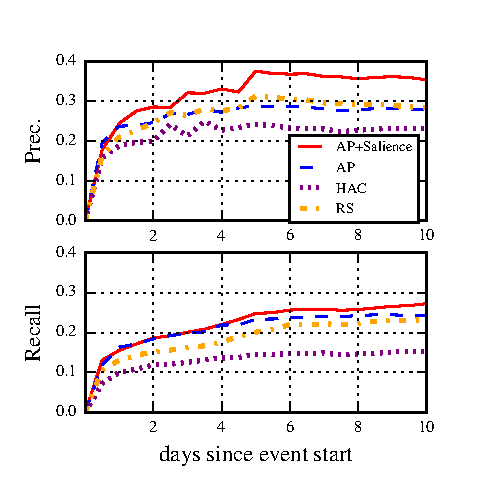
\includegraphics[]{strmsum/figures/rouge-time.eps}};
        \node[draw=white,fill=white,text width=1.05cm] at (2.20,1.55) {};
        \node[draw=white,fill=white,inner sep=0pt,text width=1.05cm] at (2.20,1.60) {\tiny SAP};
        \node[draw=white,fill=white,text width=1.05cm] at (2.20,1.30) {};
        \node[draw=white,fill=white,text width=1.05cm] at (2.20,0.95) {};
        \node[draw=white,fill=white,text width=1.05cm] at (2.20,0.55) {};

        \node[draw=white,fill=white,inner sep=0pt,text width=1.05cm] at (2.20,1.25) {\tiny AP};
        \node[draw=white,fill=white,inner sep=0pt,text width=1.05cm] at (2.20,0.90) {\tiny HAC};
        \node[draw=white,fill=white,inner sep=0pt,text width=1.05cm] at (2.20,0.55) {\tiny RS};
    \end{tikzpicture}
    \caption{System \textsc{Rouge-1} performance over time.}
\label{fig:trouge}
%\vspace{-14pt}
\end{figure}




\paragraph{\rouge} 
\autoref{tab:rouge} shows our results for system output samples against the
full summary of nuggets using \rouge. SAP improves over the individual
component systems, i.e. affinity propagation only (AP) or salience prediction
only (RS), suggesting the combination of these two components is beneficial.
This improvement is statistically significant for $\rouge-1$ and $\rouge-2$
precision, recall, and F-measures at the $\alpha = .01$ level using the
Wilcoxon signed-rank test.  The full system or the individual components AP and
RS also outperform the alternative clustering method HAC. 

SAP maintains its performance above the baselines over time as well.
\autoref{fig:trouge} shows the \rouge-1 scores over time. We show the
difference in unigram precision (bigram precision is not shown but it follows
similar curve). Within the initial days of the event, SAP is able to take the
lead over the other systems in ngram precision. The SAP model is better able to
find salient updates earlier on; for news and crisis informatics, this is an
especially important quality of the model.  Moreover, the SAP's recall is not
diminished by the high precision and remains competitive with \textsc{AP}.
Over time SAP's recall also begins to pull away, while the other models begin
to plateau.

\begin{figure}[t]
    \centering
\begin{tikzpicture}
  \node at (0,0) {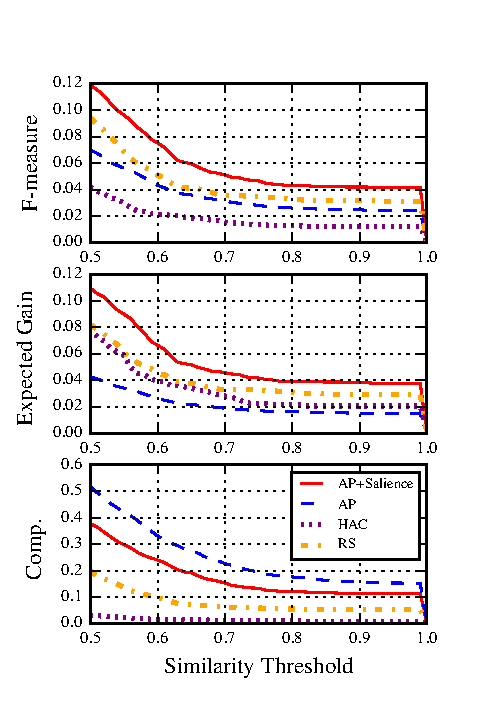
\includegraphics[]{strmsum/figures/nuggets-metrics2.eps}};
    \draw[rectangle,fill=white,draw=white] (2.85,-3.35) rectangle (1.5,-2.1); 
\node[anchor=north west, align=left,font=\tiny,inner sep=0] at (1.5,-2.1) {SAP\\[2.9pt] AP\\[2.9pt] HAC\\[2.9pt] RS};
\end{tikzpicture}
\caption{Expected Gain and Comprehensiveness performance.}
\label{fig:nperf}
%\vspace{-12pt}
\end{figure}




\paragraph{Expected Gain and Comprehensiveness}
\autoref{fig:nperf} shows the expected gain across a range of similarity
thresholds, where thresholds closer to 1 are more conservative estimates.  The
ranking of the systems remains constant across the sweep with \textsc{SAP}
beating all baseline systems. Predicting salience in general is helpful for
keeping a summary on topic as the \textsc{RS} approach outperforms the
clustering only approaches on expected gain.

When looking at the comprehensiveness of the summaries \textsc{AP} outperforms
\textsc{SAP}. The compromise encoded in the \textsc{SAP} objective function,
between being representative and being salient, is seen clearly here where the
performance of the \textsc{SAP} methods is lower bounded by the salience
focused \textsc{RS} system and upper bounded by the clustering only \textsc{AP}
system. Overall, \textsc{SAP} achieves the best balance of these two metrics.

\subsection{Feature Ablation}
\begin{table}[h]
\centering
% centering table
\begin{tabular}{l D{.}{.}{3} D{.}{.}{3} D{.}{.}{3} D{.}{.}{3} D{.}{.}{3} D{.}{.}{3}}
    \toprule
% creating 10 columns
    & \multicolumn{3}{c}{\textsc{Rouge}-1}
    & \multicolumn{3}{c}{\textsc{Rouge}-2}\\
    \cmidrule(lr){2-4} \cmidrule(lr){5-7}
    Model & \multicolumn{1}{c}{Recall} & \multicolumn{1}{c}{Prec.} & \multicolumn{1}{c}{$\textrm{F}_1$} &
\multicolumn{1}{c}{Recall} & \multicolumn{1}{c}{Prec.} & \multicolumn{1}{c}{$\textrm{F}_1$} \\
\midrule
Full System & 0.282 & 0.344 & 0.306 & 0.045 & 0.056 & 0.049\\
No Basic    & 0.263 & 0.380 \rlap{\textsuperscript{$\dagger$}}  & 0.294 & 0.046 & 0.068 \rlap{\textsuperscript{$\dagger\dagger$}} & 0.051 \rlap{\textsuperscript{$\dagger$}}\\
No LM       & 0.223 \rlap{\textsuperscript{$\dagger$}} & 0.361 & 0.254 \rlap{\textsuperscript{$\dagger$}} & 0.033 \rlap{\textsuperscript{$\dagger$}} & 0.056 & 0.038 \rlap{\textsuperscript{$\dagger$}} \\
No Time  & 0.297 \rlap{\textsuperscript{$\dagger$}} & 0.367 \rlap{\textsuperscript{$\dagger\dagger$}} & 0.322 \rlap{\textsuperscript{$\dagger$}} & 0.052 \rlap{\textsuperscript{$\dagger\dagger$}} & 0.064 \rlap{\textsuperscript{$\dagger\dagger$}} & 0.056 \rlap{\textsuperscript{$\dagger\dagger$}} \\ 
No Geo   & 0.232 \rlap{\textsuperscript{$\dagger\dagger$}} & 0.381 & 0.265 \rlap{\textsuperscript{$\dagger$}} & 0.037 \rlap{\textsuperscript{$\dagger$}} & 0.065 & 0.042 \\  
No Query & 0.251 & 0.377 & 0.280 & 0.043 & 0.068 \rlap{\textsuperscript{$\dagger$}} & 0.048 \\
\bottomrule
\end{tabular}
\caption{Feature ablation \textsc{Rouge} performance. 
    $\dagger$ indicates statistically significant difference from 
full model at the $\alpha=.05$ level.
    $\dagger\dagger$ indicates statistically significant difference from 
full model at the $\alpha=.01$ level.
    } % title name of the table
\label{tab:farouge}
\end{table}








\autoref{tab:farouge} shows the results of our feature ablation tests.
Removing the language models yields a statistically significant drop in both
ngram recall and F-measure. 

Removing the language model and geographic relevance features leads to a
statistically significant drop in \rouge-1 F1 scores. Unfortunately, this is
not the case for the temporal relevance features. We surmise that these
features are too strongly correlated with each other, i.e. the differences in
TF-IDF between hours are definitely not i.i.d.  variables. 

Interestingly, removing the basic features leads to an increase in both unigram
and bigram precision; in the bigram case this is enough to cause a
statistically significant increase in F-measure over the full model. In other
words, the generic features actually lead to an inferior model when we can
incorporate more appropriate domain specific features.  This result perhaps
echoes the claim of \cite{jones1999} that generic approaches to summarization
are unlikely to produce truly useful summaries.
